% !TeX document-id = {b018c267-2972-4b88-832a-8761fc6fabcf}
% !BIB TS-program = biber
\documentclass[xetex,aspectratio=169]{beamer}

\usepackage[spanish,english]{babel}
\usepackage{graphicx}
\usepackage{graphicx}
\usepackage{hyperref}
\usepackage{tikz}
\usepackage{csquotes}
%\usepackage{natbib}
\usepackage[style=authoryear, backend=biber]{biblatex}
\addbibresource{biblio.bib}
\usepackage{caption}
\usepackage{subcaption}
\usepackage{amsmath}
\usepackage{url}
\usepackage[bigfiles]{pdfbase}

\usetikzlibrary{shapes, arrows, positioning, calc}  
\usetikzlibrary{overlay-beamer-styles}


\usetheme{modern}

\newcommand{\mypos}[2]{\tikz[remember picture]{\node[inner sep=0pt, anchor=base](#2){#1};}}
%\setcitestyle{authoryear,open={(},close={)}}
\DeclareMathOperator*{\argmin}{arg\,min}
\renewcommand*{\nameyeardelim}{\addcomma\space}

\newcommand{\implyarrow}{%
	\mathrel{\raisebox{1.3ex}{\rotatebox[origin=c]{90}{\mathhexbox37F}}}}

\tikzset{%
	block/.style    = {rounded corners, draw, thick, circle, minimum height = 3em,
		minimum width = 3em, fill = yellow!50},
	point/.style    = {coordinate}, % Input
}

\ExplSyntaxOn
\NewDocumentCommand\embedvideo{smm}{
	\group_begin:
	\leavevmode
	\tl_if_exist:cTF{file_\file_mdfive_hash:n{#3}}{
		\tl_set_eq:Nc\video{file_\file_mdfive_hash:n{#3}}
	}{
		\IfFileExists{#3}{}{\GenericError{}{File~`#3'~not~found}{}{}}
		\pbs_pdfobj:nnn{}{fstream}{{}{#3}}
		\pbs_pdfobj:nnn{}{dict}{
			/Type/Filespec/F~(#3)/UF~(#3)
			/EF~<</F~\pbs_pdflastobj:>>
		}
		\tl_set:Nx\video{\pbs_pdflastobj:}
		\tl_gset_eq:cN{file_\file_mdfive_hash:n{#3}}\video
	}
	%
	\pbs_pdfobj:nnn{}{dict}{
		/Type/RichMediaInstance/Subtype/Video
		/Asset~\video
		/Params~<</FlashVars (
		source=#3&
		skin=SkinOverAllNoFullNoCaption.swf&
		skinAutoHide=true&
		skinBackgroundColor=0x5F5F5F&
		skinBackgroundAlpha=0.75&
		loop=true
		)>>
	}
	%
	\pbs_pdfobj:nnn{}{dict}{
		/Type/RichMediaConfiguration/Subtype/Video
		/Instances~[\pbs_pdflastobj:]
	}
	%
	\pbs_pdfobj:nnn{}{dict}{
		/Type/RichMediaContent
		/Assets~<<
		/Names~[(#3)~\video]
		>>
		/Configurations~[\pbs_pdflastobj:]
	}
	\tl_set:Nx\rmcontent{\pbs_pdflastobj:}
	%
	\pbs_pdfobj:nnn{}{dict}{
		/Activation~<<
		/Condition/\IfBooleanTF{#1}{PV}{XA}
		/Presentation~<</Style/Embedded>>
		>>
		/Deactivation~<</Condition/PI>>
	}
	%
	\hbox_set:Nn\l_tmpa_box{#2}
	\tl_set:Nx\l_box_wd_tl{\dim_use:N\box_wd:N\l_tmpa_box}
	\tl_set:Nx\l_box_ht_tl{\dim_use:N\box_ht:N\l_tmpa_box}
	\tl_set:Nx\l_box_dp_tl{\dim_use:N\box_dp:N\l_tmpa_box}
	\pbs_pdfxform:nnnnn{1}{1}{}{}{\l_tmpa_box}
	%
	\pbs_pdfannot:nnnn{\l_box_wd_tl}{\l_box_ht_tl}{\l_box_dp_tl}{
		/Subtype/RichMedia
		/BS~<</W~0/S/S>>
		/Contents~(embedded~video~file:#3)
		/NM~(rma:#3)
		/AP~<</N~\pbs_pdflastxform:>>
		/RichMediaSettings~\pbs_pdflastobj:
		/RichMediaContent~\rmcontent
	}
	\phantom{#2}
	\group_end:
}
\ExplSyntaxOff


\title
    {Desde los campos magnéticos hasta la formación de planetas}
\subtitle
    {Desentrañando los misterios del universo con big computing y big data}
\author
    {Miguel Cárcamo}

\date[03-05-2023]{3 de Mayo de 2023}

\institute[USACH]{Universidad de Santiago de Chile}


\begin{document}

    \frame[plain]{\titlepage}
	\section{Espectro electromagnético}
	{
	\setbeamertemplate{background canvas}{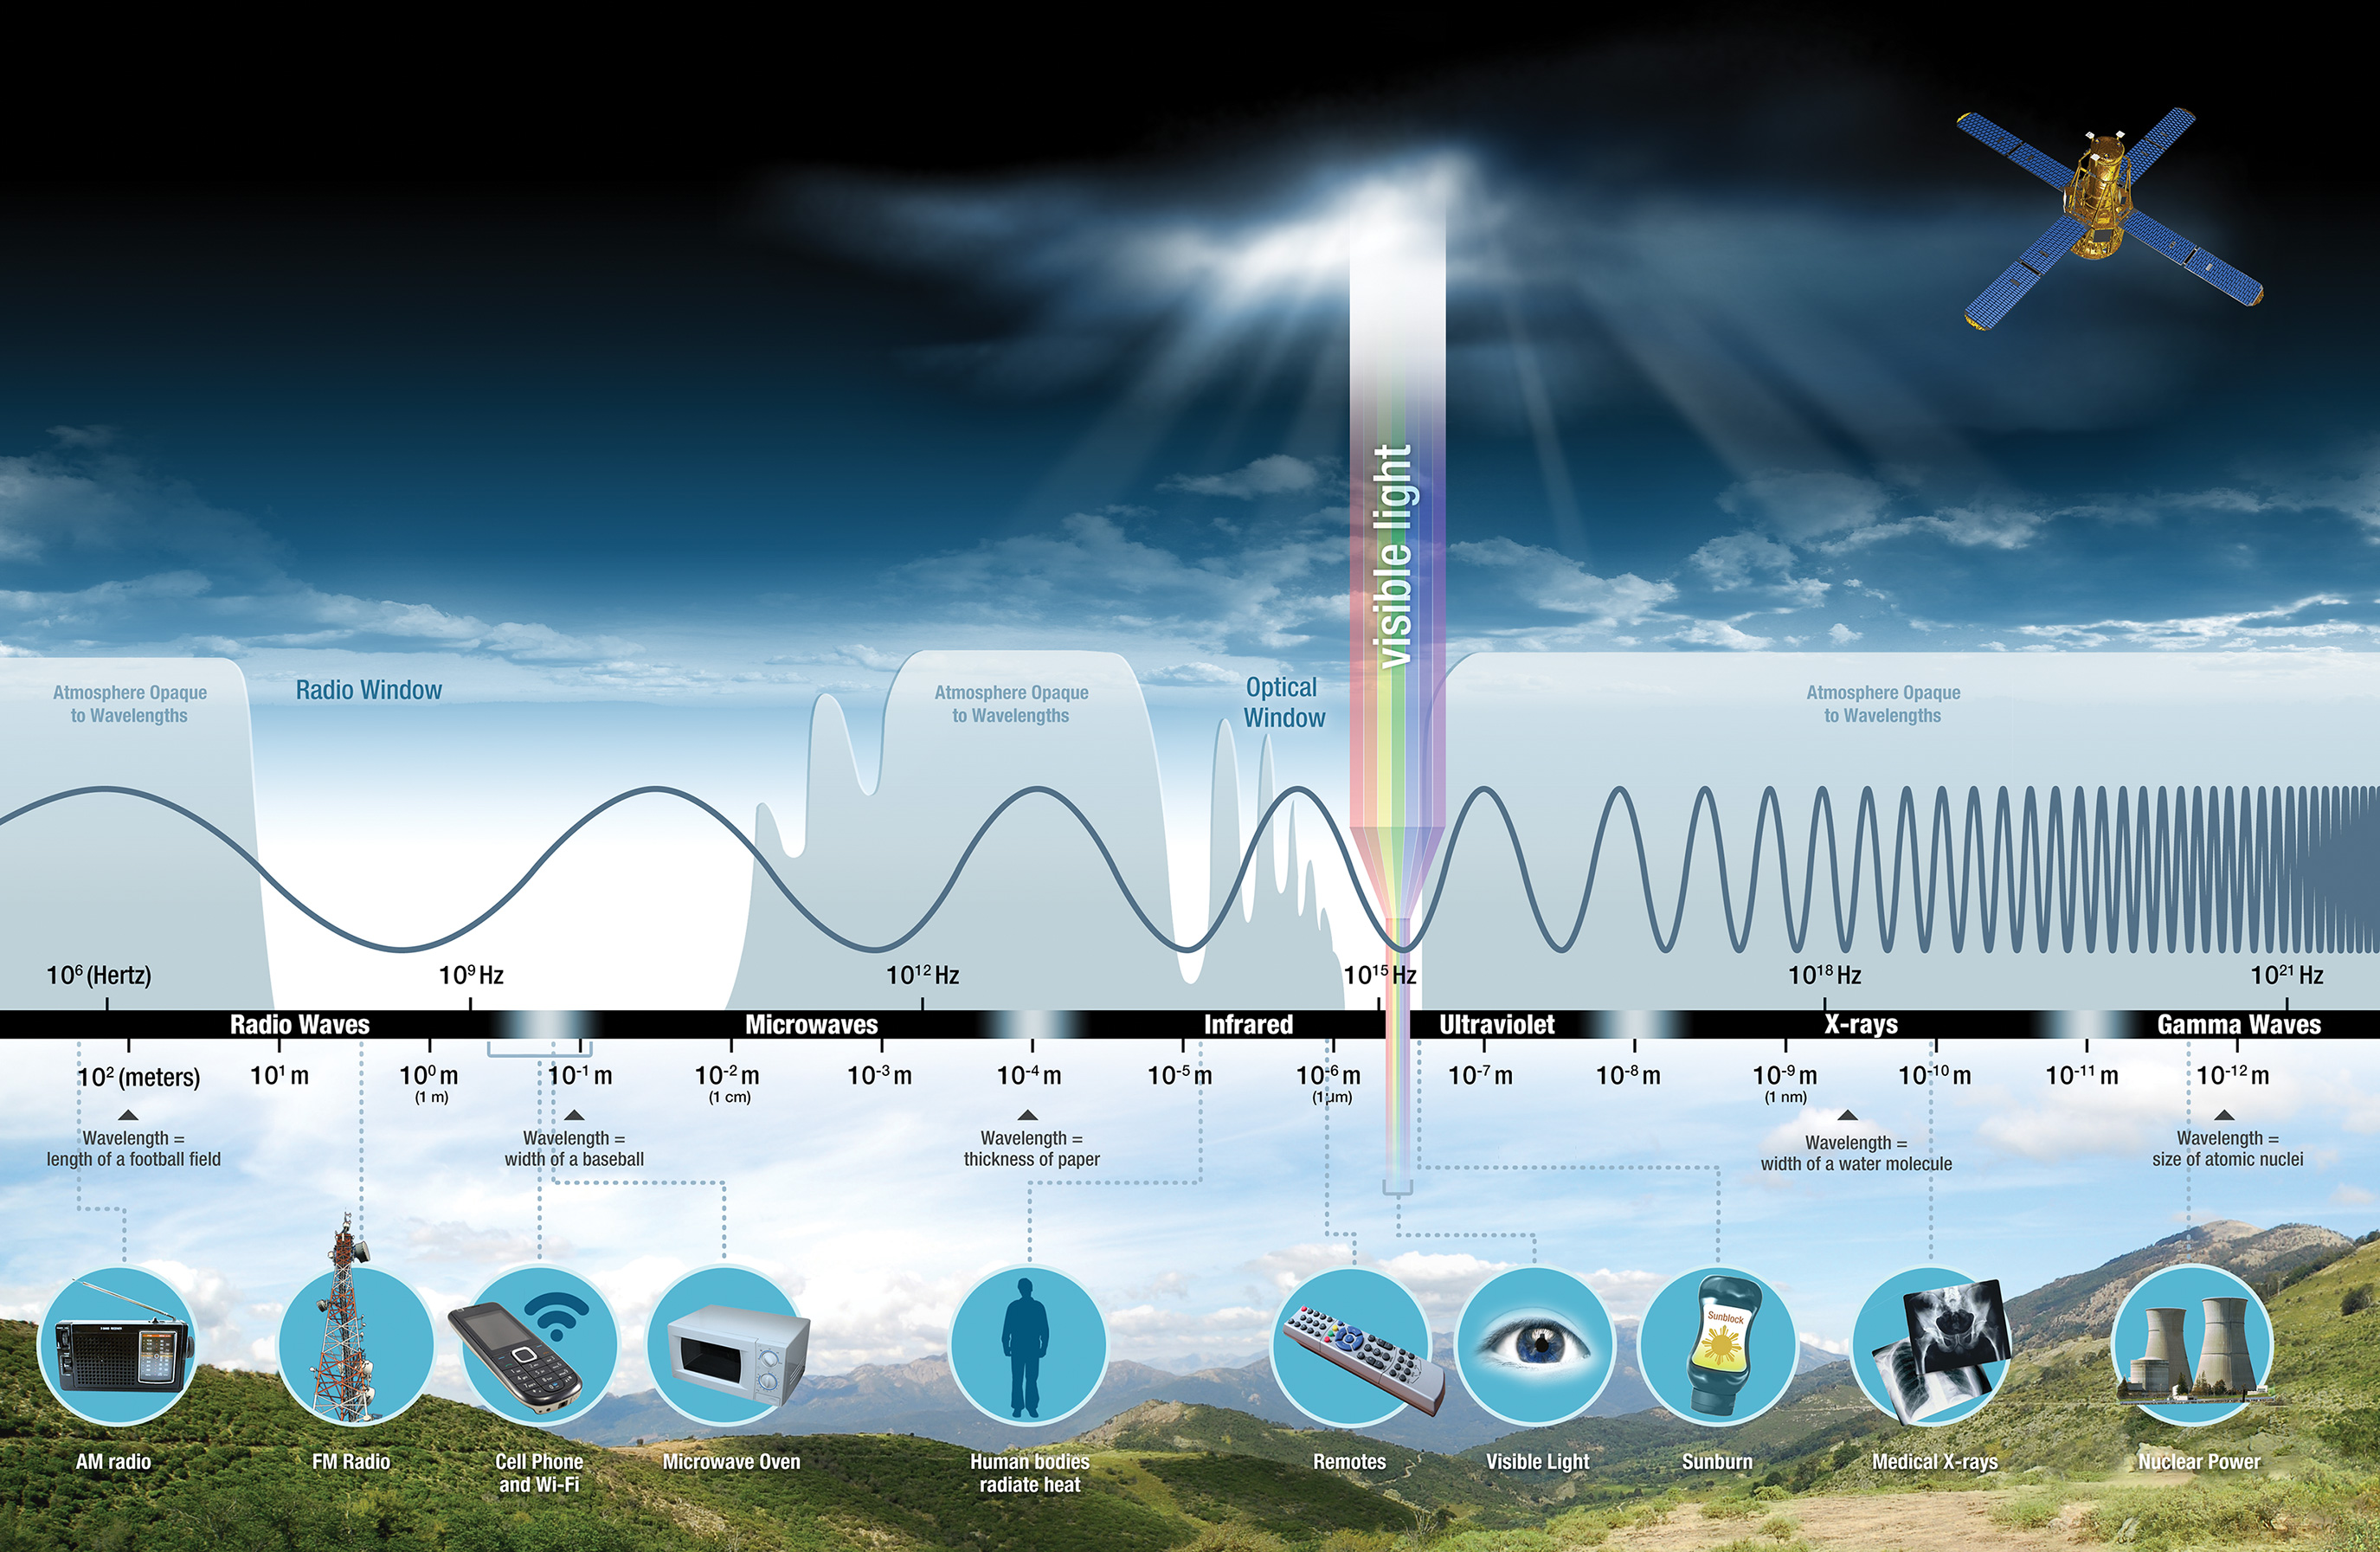
\includegraphics[height = \paperheight, 
		width = \paperwidth]{./figures/electro_spectrum/EMS-Introduction}}
	\begin{frame}{}
	\end{frame}
	}
	%\begin{frame}{Espectro electromagnético}
	%	\begin{figure}
	%		\centering
	%		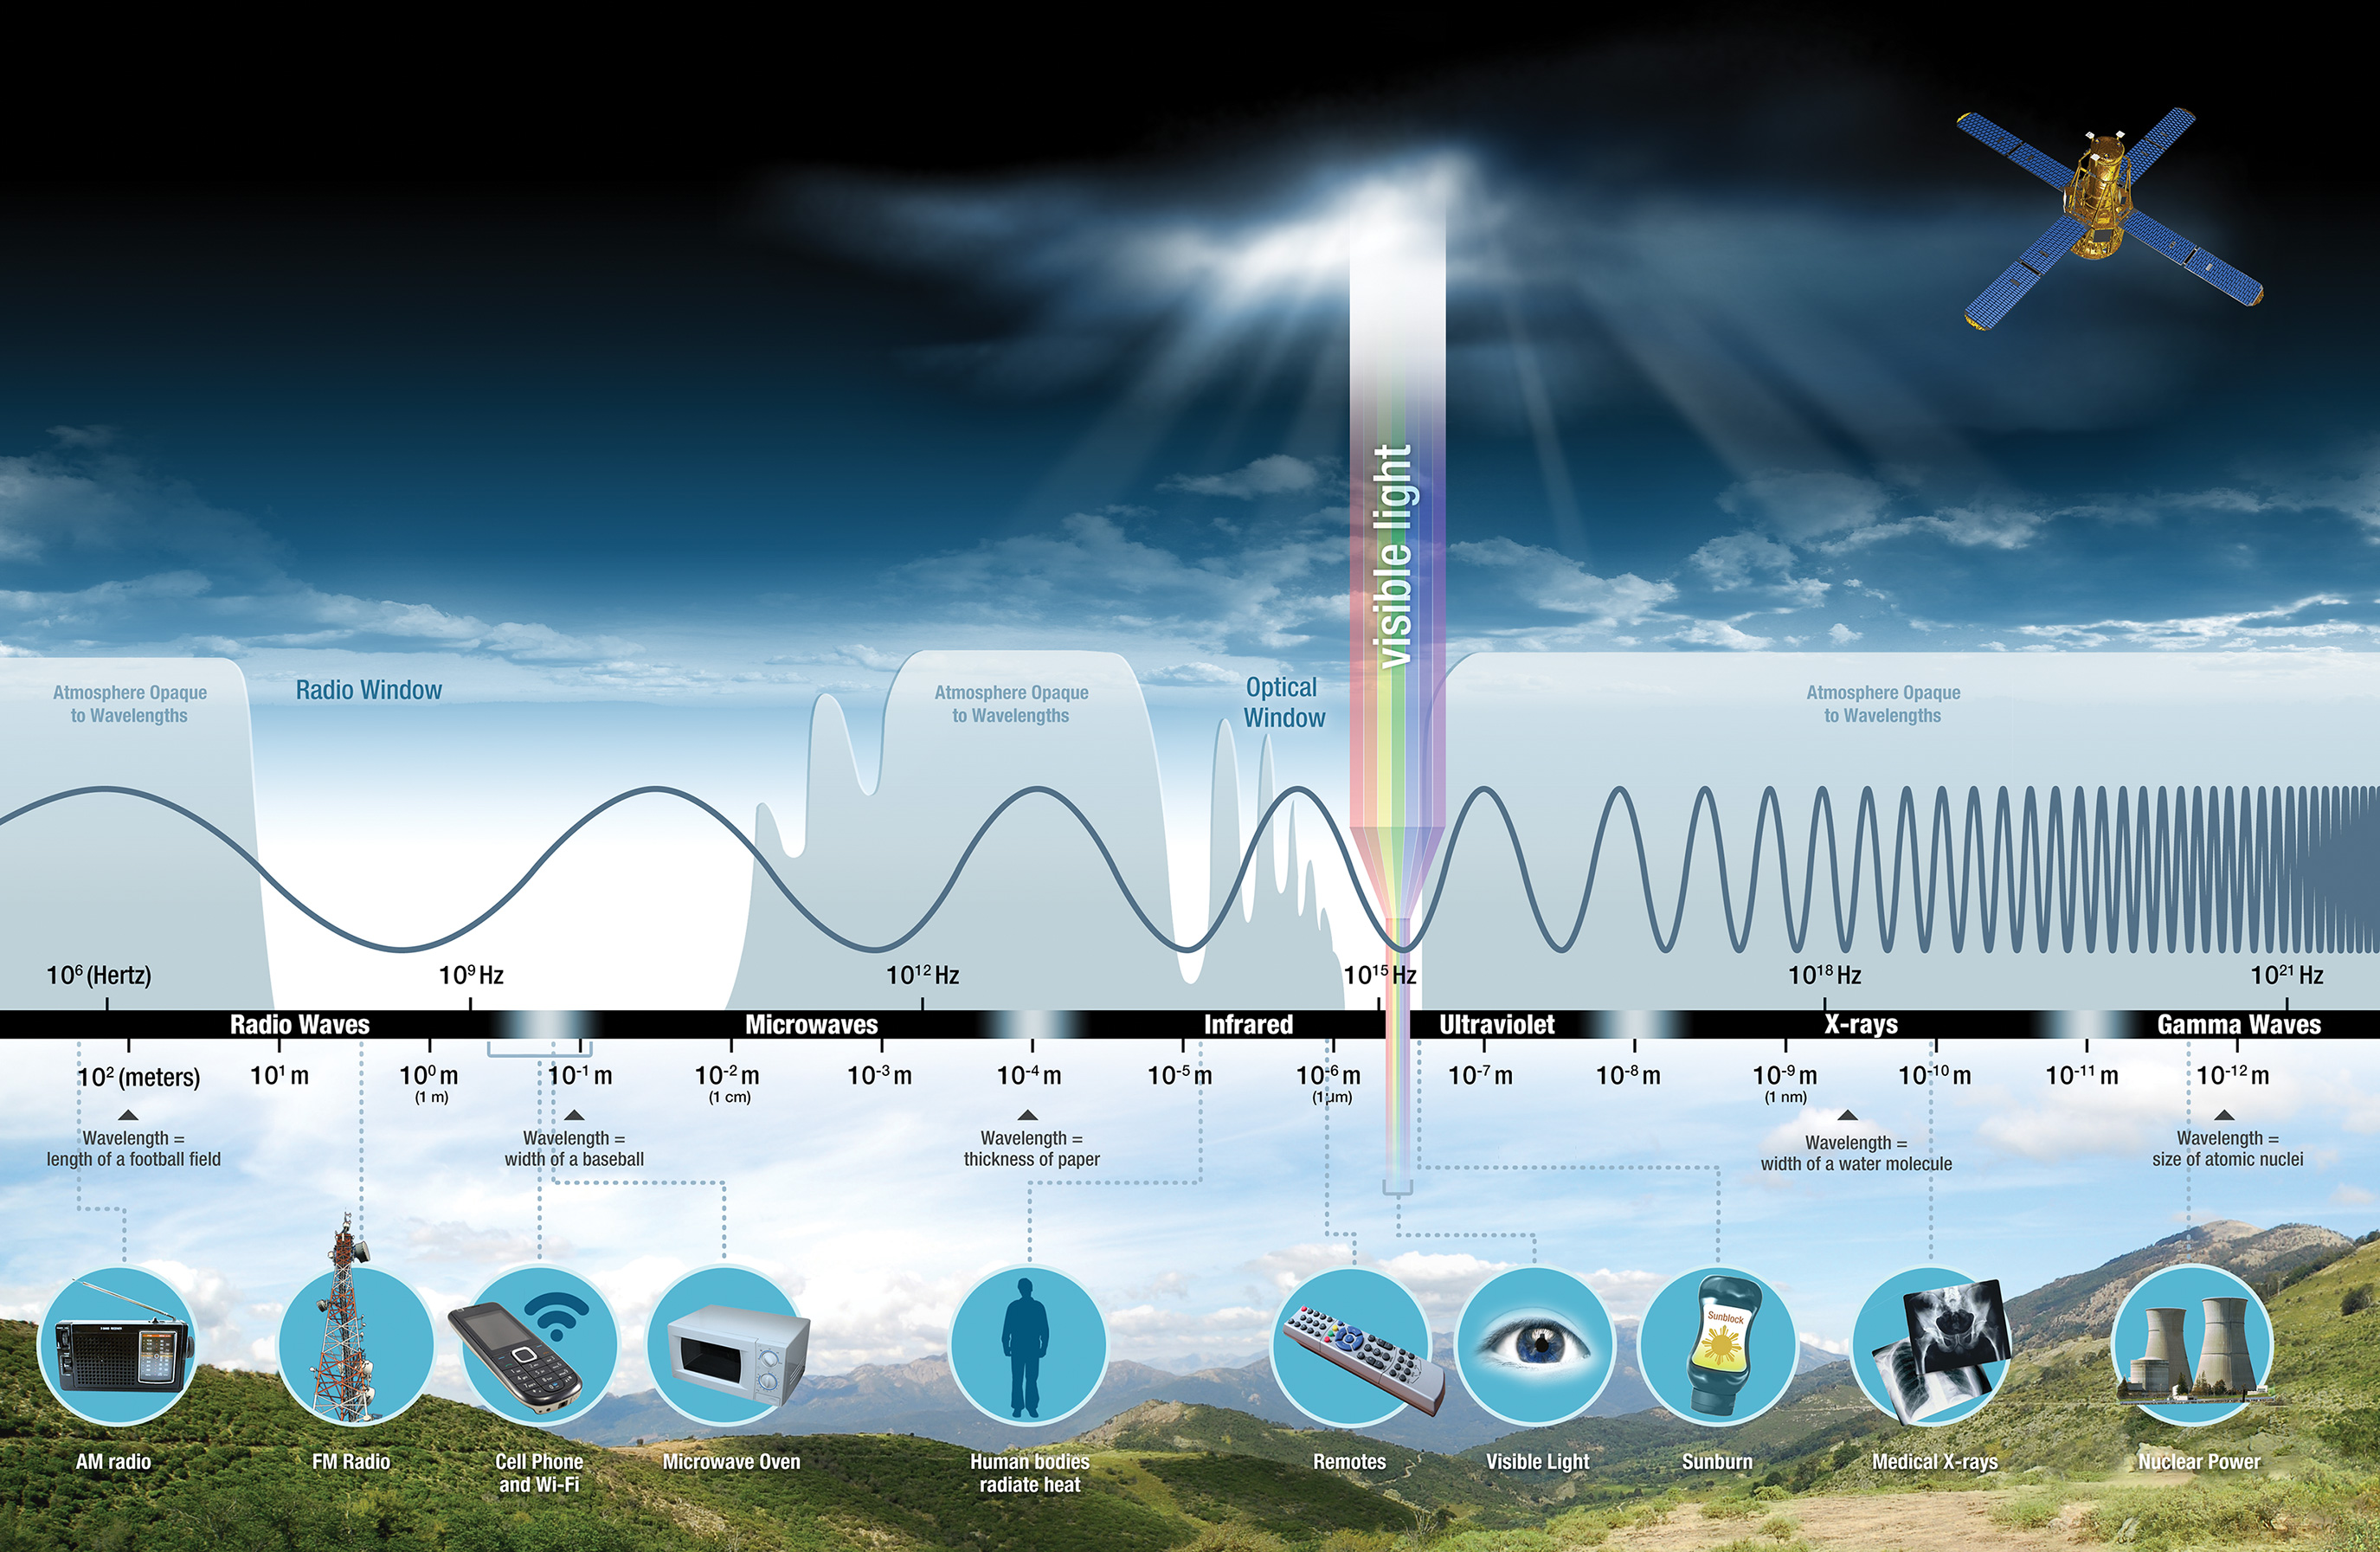
\includegraphics[width=\textwidth, height=.8\textheight, keepaspectratio]{./figures/electro_spectrum/EMS-Introduction}
	%		\caption{Espectro electromagnético, NASA}
	%	\end{figure}
	%\end{frame}

	\begin{frame}{Espectro electromagnético}
		\begin{columns}
			\begin{column}{0.48\textwidth}
				\begin{figure}
					\centering
					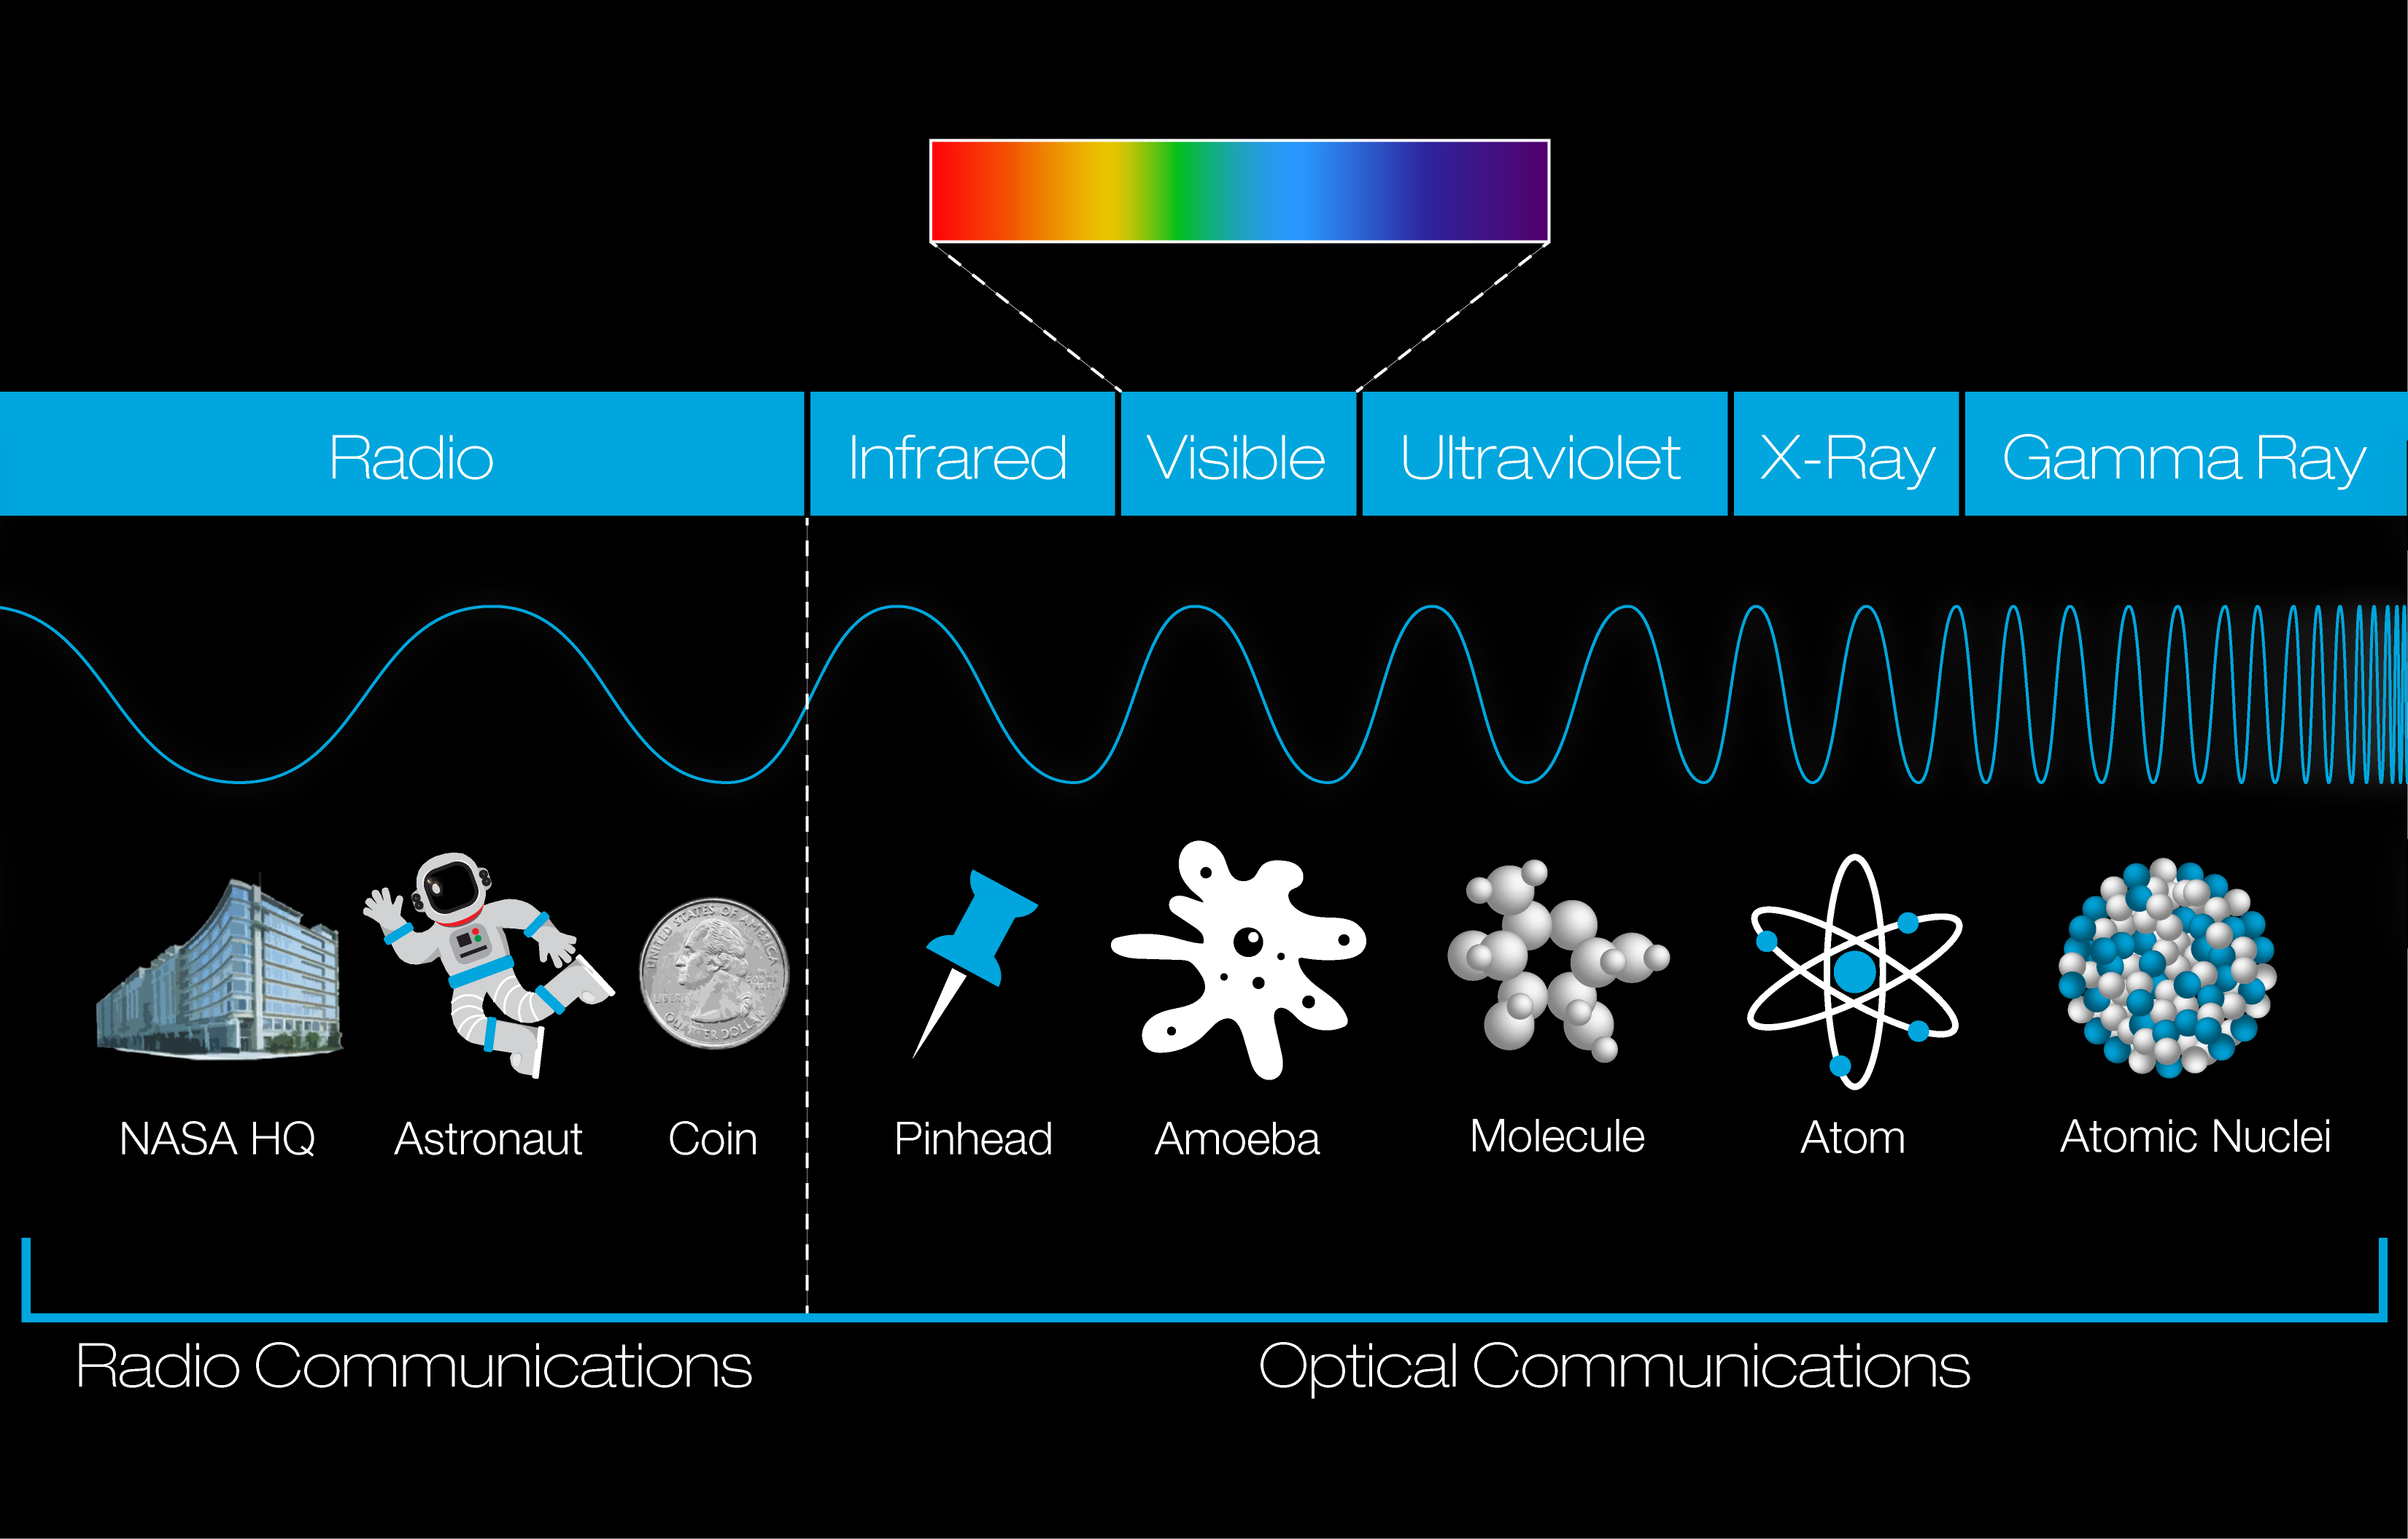
\includegraphics[width=\textwidth, keepaspectratio]{./figures/electro_spectrum/spectrum_radio_waves_graphic_web_0}
					\caption{Espectro electromagnético, NASA}
				\end{figure}
			\end{column}
			\begin{column}{0.48\textwidth}
				\begin{figure}
					\centering
					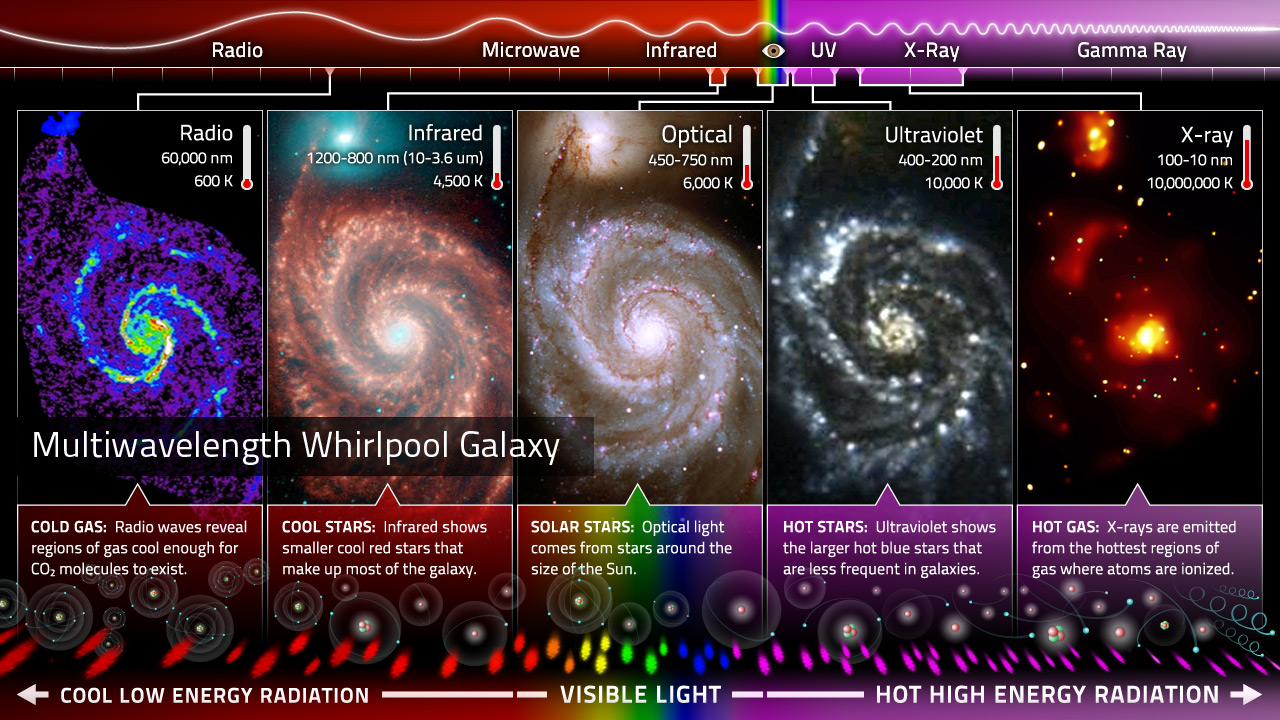
\includegraphics[width=\textwidth, keepaspectratio]{./figures/electro_spectrum/MWA-whirlpool-galaxy}
					\caption{Espectro electromagnético, NASA y University of Chicago}
				\end{figure}
			\end{column}
		\end{columns}
		
	\end{frame}

	\begin{frame}{Como funcionan los radio interferometros}
		content...
	\end{frame}
	
    \section{Radio interferometría}
    \begin{frame}{Atacama Large Telescope Array (ALMA)}
    	\begin{columns}
    		\begin{column}{0.48\textwidth}
    			\begin{itemize}
    				\item 66 antenas
    				\begin{itemize}
    					\item 50 - 12m de diametro
    					\item 12 - 7m de diametro
    					\item 4 - 12m de diametro
    				\end{itemize}
    				\item Minimo baseline de 15m
    				\item Máximo baseline de 16km
    				\item Longitudes de onda desde 6 a 0.32 mm (35-950 GHz)
    			\end{itemize}
    		\end{column}
    		\begin{column}{0.48\textwidth}
    			\begin{figure}
    				\centering		
    				\embedvideo*{\includegraphics[page=1, width=\textwidth, height=0.8\textheight, keepaspectratio]{example-movie}}{./videos/alma_1.mp4}
    				\caption{Antenas ALMA, ALMA NRAO Outreach}
    		\end{figure}
    		\end{column}
    	\end{columns}
    \end{frame}

	\begin{frame}{Square Kilometre Array (SKA)}
		\begin{columns}
			\begin{column}{0.48\textwidth}
				\begin{figure}
					\centering
					\begin{subfigure}[b]{\textwidth}
						\centering
						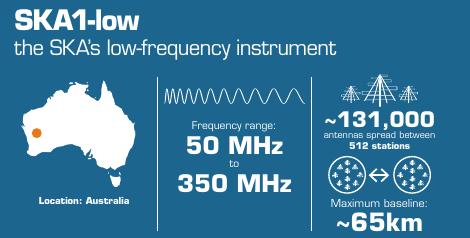
\includegraphics[width=\textwidth, height=0.41\textheight, keepaspectratio]{./figures/ska/ska_low.png}
						%\caption{Filaments}
						%\label{fig:skalow}
					\end{subfigure}
					
					\begin{subfigure}[b]{\textwidth}
						\centering
						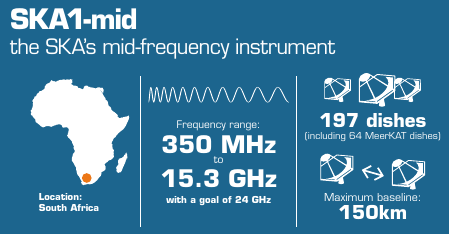
\includegraphics[width=\textwidth, height=0.41\textheight, keepaspectratio]{./figures/ska/ska_mid.png}
						%\caption{Galaxy cluster}
						%\label{fig:skamid}
					\end{subfigure}
				\end{figure}
			\end{column}
			\begin{column}{0.48\textwidth}
				\embedvideo*{\includegraphics[page=1, width=\textwidth, height=0.4\textheight, keepaspectratio]{example-movie}}{./videos/skalow.mp4}
				\embedvideo*{\includegraphics[page=1, width=\textwidth, height=0.4\textheight, keepaspectratio]{example-movie}}{./videos/skamid.mp4}
			\end{column}
		\end{columns}
	\end{frame}

	\begin{frame}{SKA Science goals}
		\begin{figure}
			\subfloat[First black holes and stars]{\embedvideo*{\includegraphics[page=1, width=.225\linewidth, keepaspectratio]{example-movie}}{./videos/ska_1.mp4}}\hfill
			\subfloat[Galaxy evolution and dark energy]{\embedvideo*{\includegraphics[page=1, width=.225\linewidth, keepaspectratio]{example-movie}}{./videos/ska_2.mp4}}\hfill
			\subfloat[Gravitational waves]{\embedvideo*{\includegraphics[page=1, width=.225\linewidth, keepaspectratio]{example-movie}}{./videos/ska_3.mp4}}\hfill
			%\bigskip
			
			\subfloat[Cosmic magnetic fields]{\embedvideo*{\includegraphics[page=1,width=.225\linewidth, keepaspectratio]{example-movie}}{./videos/ska_4.mp4}}\hfill
			\subfloat[Are we alone?]{\embedvideo*{\includegraphics[page=1, width=.225\linewidth, keepaspectratio]{example-movie}}{./videos/ska_5.mp4}}\hfill
			\caption{SKA Science goals, SKAO}
		\end{figure}
	\end{frame}

	\section{Historia del universo}
	{
	\setbeamertemplate{background canvas}{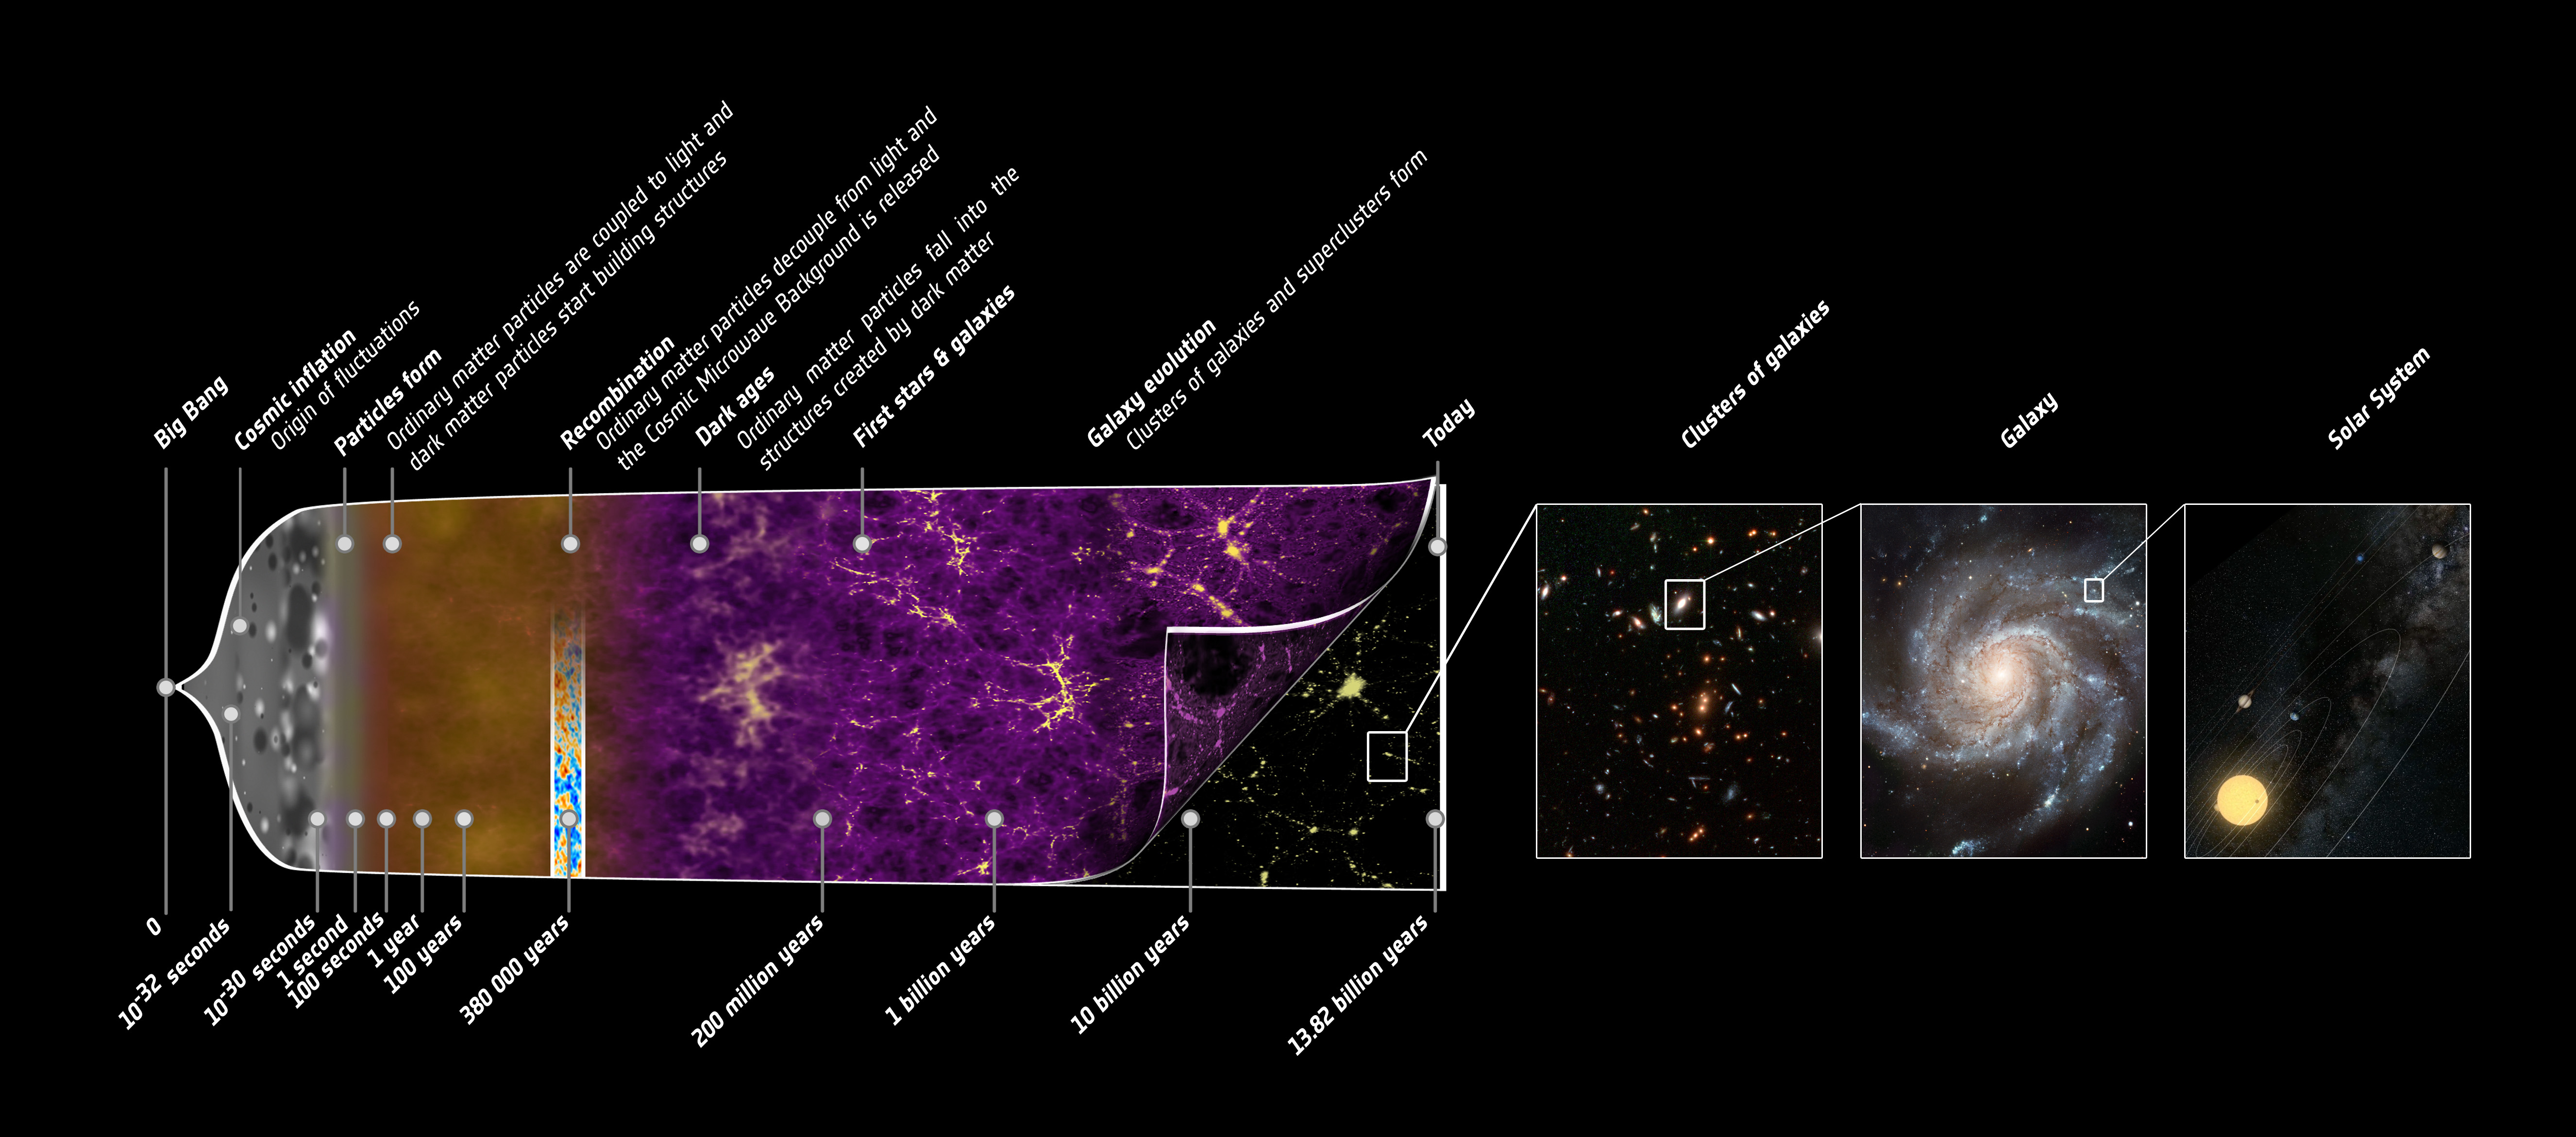
\includegraphics[height = \paperheight, 
		width = \paperwidth]{./figures/universe/universe}}
	\begin{frame}{}
	\end{frame}
	}

	\section{Campos magnéticos cósmicos}
	\begin{frame}{Campos magnéticos cósmicos}
		\begin{columns}
			
			\begin{column}{0.48\textwidth}
				\begin{itemize}
					\item Evolución de galaxias
					\item Formación de estrellas
					\item Remanentes de supernovas
					\item Su origen es \alert{\textbf{DESCONOCIDO}}
				\end{itemize}
				\begin{itemize}
					\item Dos maneras de estudiarlos:
					\begin{itemize}
						\item Filamentos en vacíos
						\item Cúmulos de galaxias
					\end{itemize}
				\end{itemize}
			\end{column}
			
			\begin{column}{0.48\textwidth}
				
				\embedvideo*{\includegraphics[page=1, width=\textwidth, height=0.5\textheight, keepaspectratio]{example-movie}}{./videos/ska_4.mp4}
				
			\end{column}
		\end{columns}
	\end{frame}
	
	\begin{frame}{Campos magnéticos cósmicos}
		\begin{columns}
			
			\begin{column}{0.48\textwidth}
				\begin{itemize}
					\item Evolución de galaxias
					\item Formación de estrellas
					\item Remanentes de supernovas
					\item Su origen es \alert{\textbf{DESCONOCIDO}}
				\end{itemize}
				\begin{itemize}
					\item Dos maneras de estudiarlos:
					\begin{itemize}
						\item Filamentos en vacíos
						\item Cúmulos de galaxias
					\end{itemize}
				\end{itemize}
			\end{column}
			
			\begin{column}{0.48\textwidth}
				
				\embedvideo*{\includegraphics[page=1, width=\textwidth, height=0.4\textheight, keepaspectratio]{example-movie}}{./videos/gclusters.mp4}
				\embedvideo*{\includegraphics[page=1, width=\textwidth, height=0.4\textheight, keepaspectratio]{example-movie}}{./videos/cosmic_web.mp4}
				
			\end{column}
		\end{columns}
	\end{frame}
	
	\section{Radiacion sincrotron}
	\begin{frame}{Radiacion sincrotron}
		\begin{columns}
			
			\begin{column}{0.48\textwidth}
				\begin{figure}
					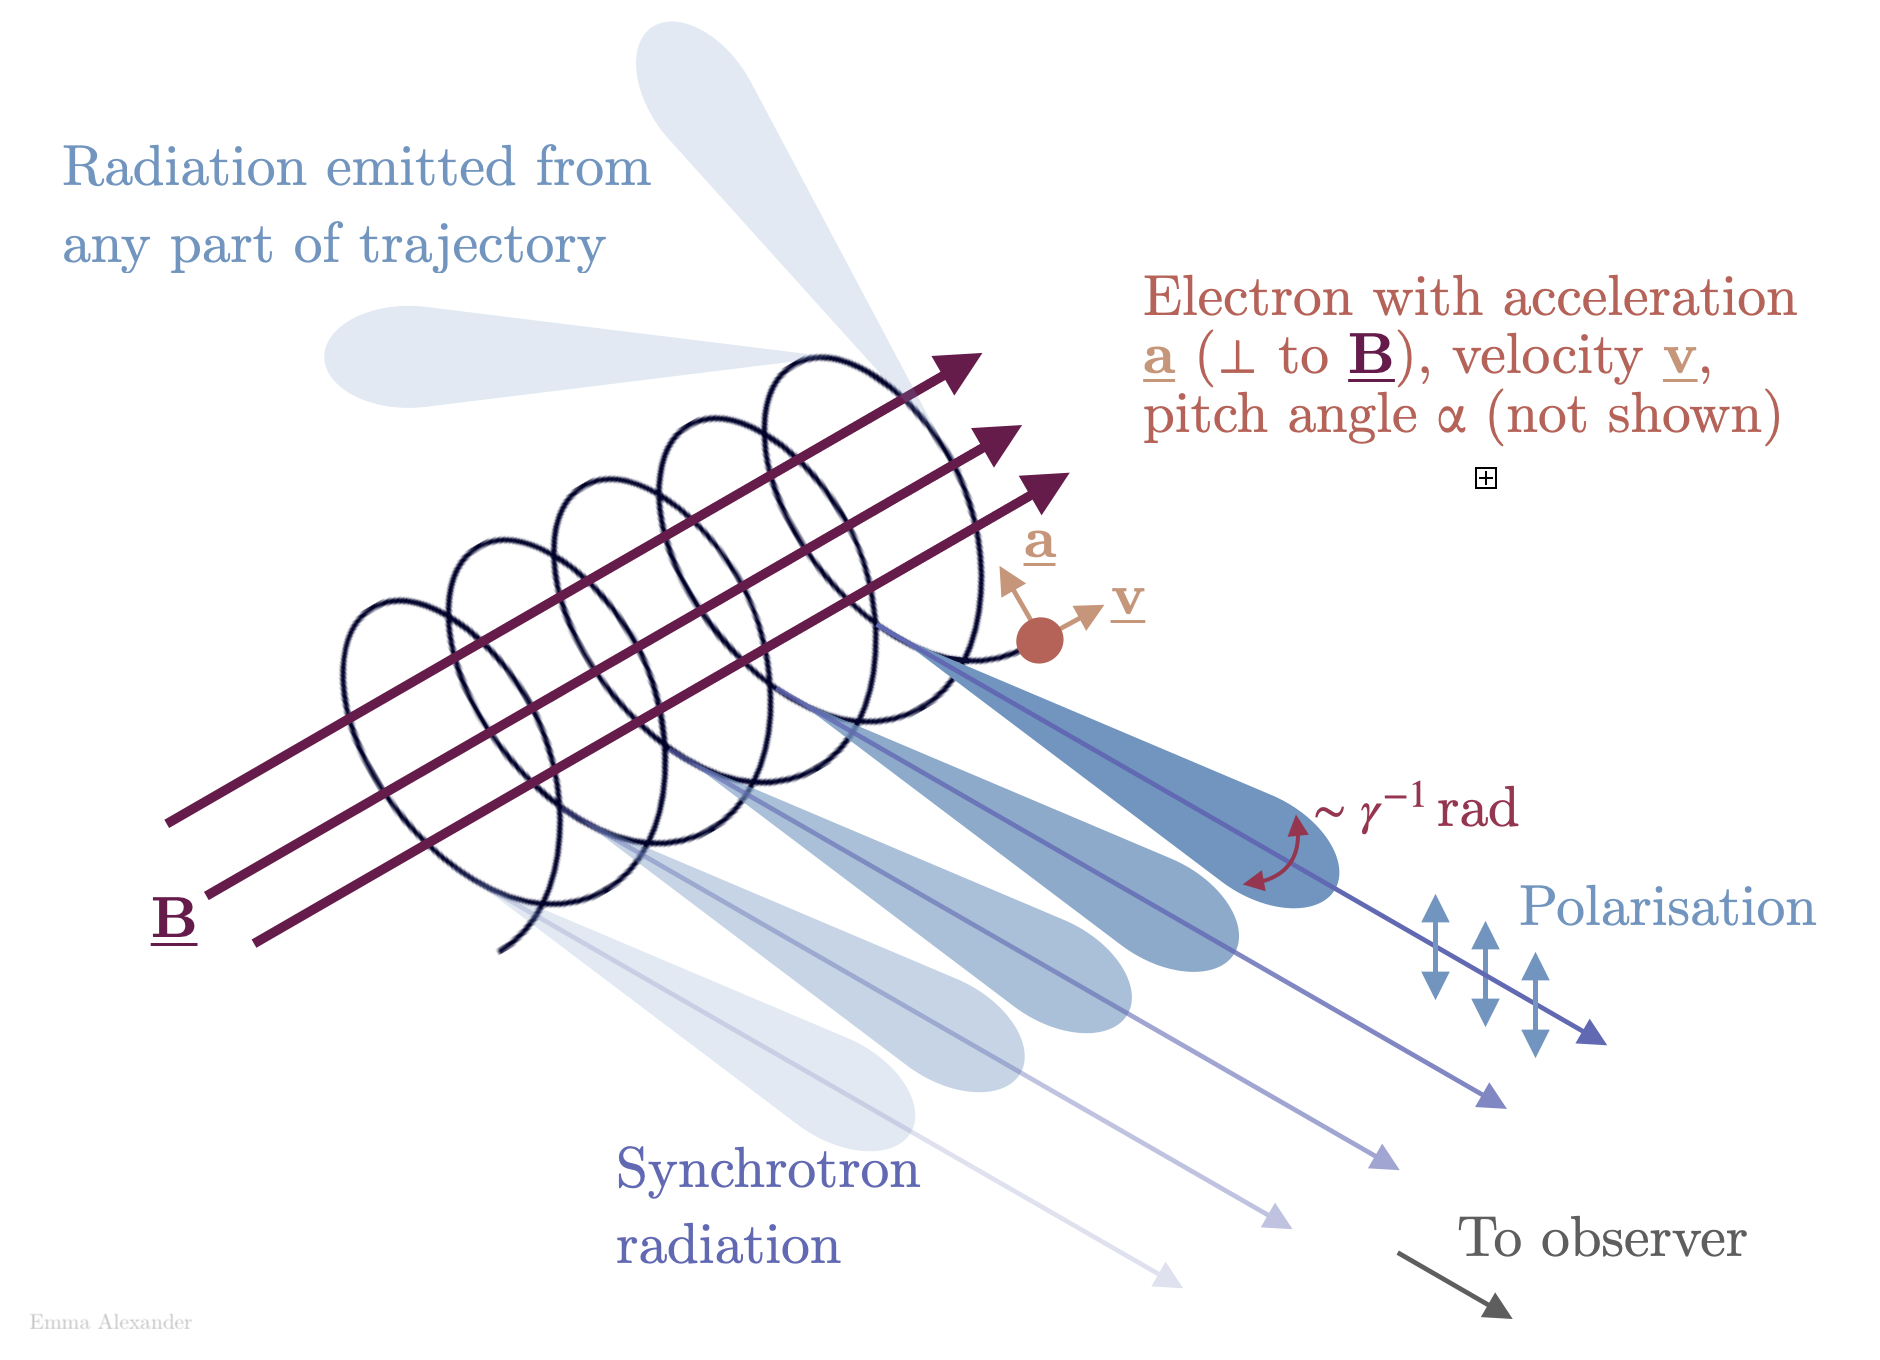
\includegraphics[width=\textwidth, keepaspectratio]{./figures/synchrotron/synchrotron.png}
					\caption{Mecanismo de radiacion sincrotron, Emma Alexander.}
				\end{figure}
			\end{column}
			
			\begin{column}{0.48\textwidth}
				\begin{figure}
					\embedvideo*{\includegraphics[page=1, width=\textwidth, keepaspectratio]{example-movie}}{./videos/agn.mp4}
					\caption{3C120 (Concepcion artistica), Marscher et al., Wolfgang Steffen, Cosmovision, NRAO/AUI/NSF}
				\end{figure}
				
				
			\end{column}
		\end{columns}
	\end{frame}
	
	\begin{frame}{Radiacion sincrotron}
		\begin{columns}
			
			\begin{column}{0.48\textwidth}
				\begin{figure}
					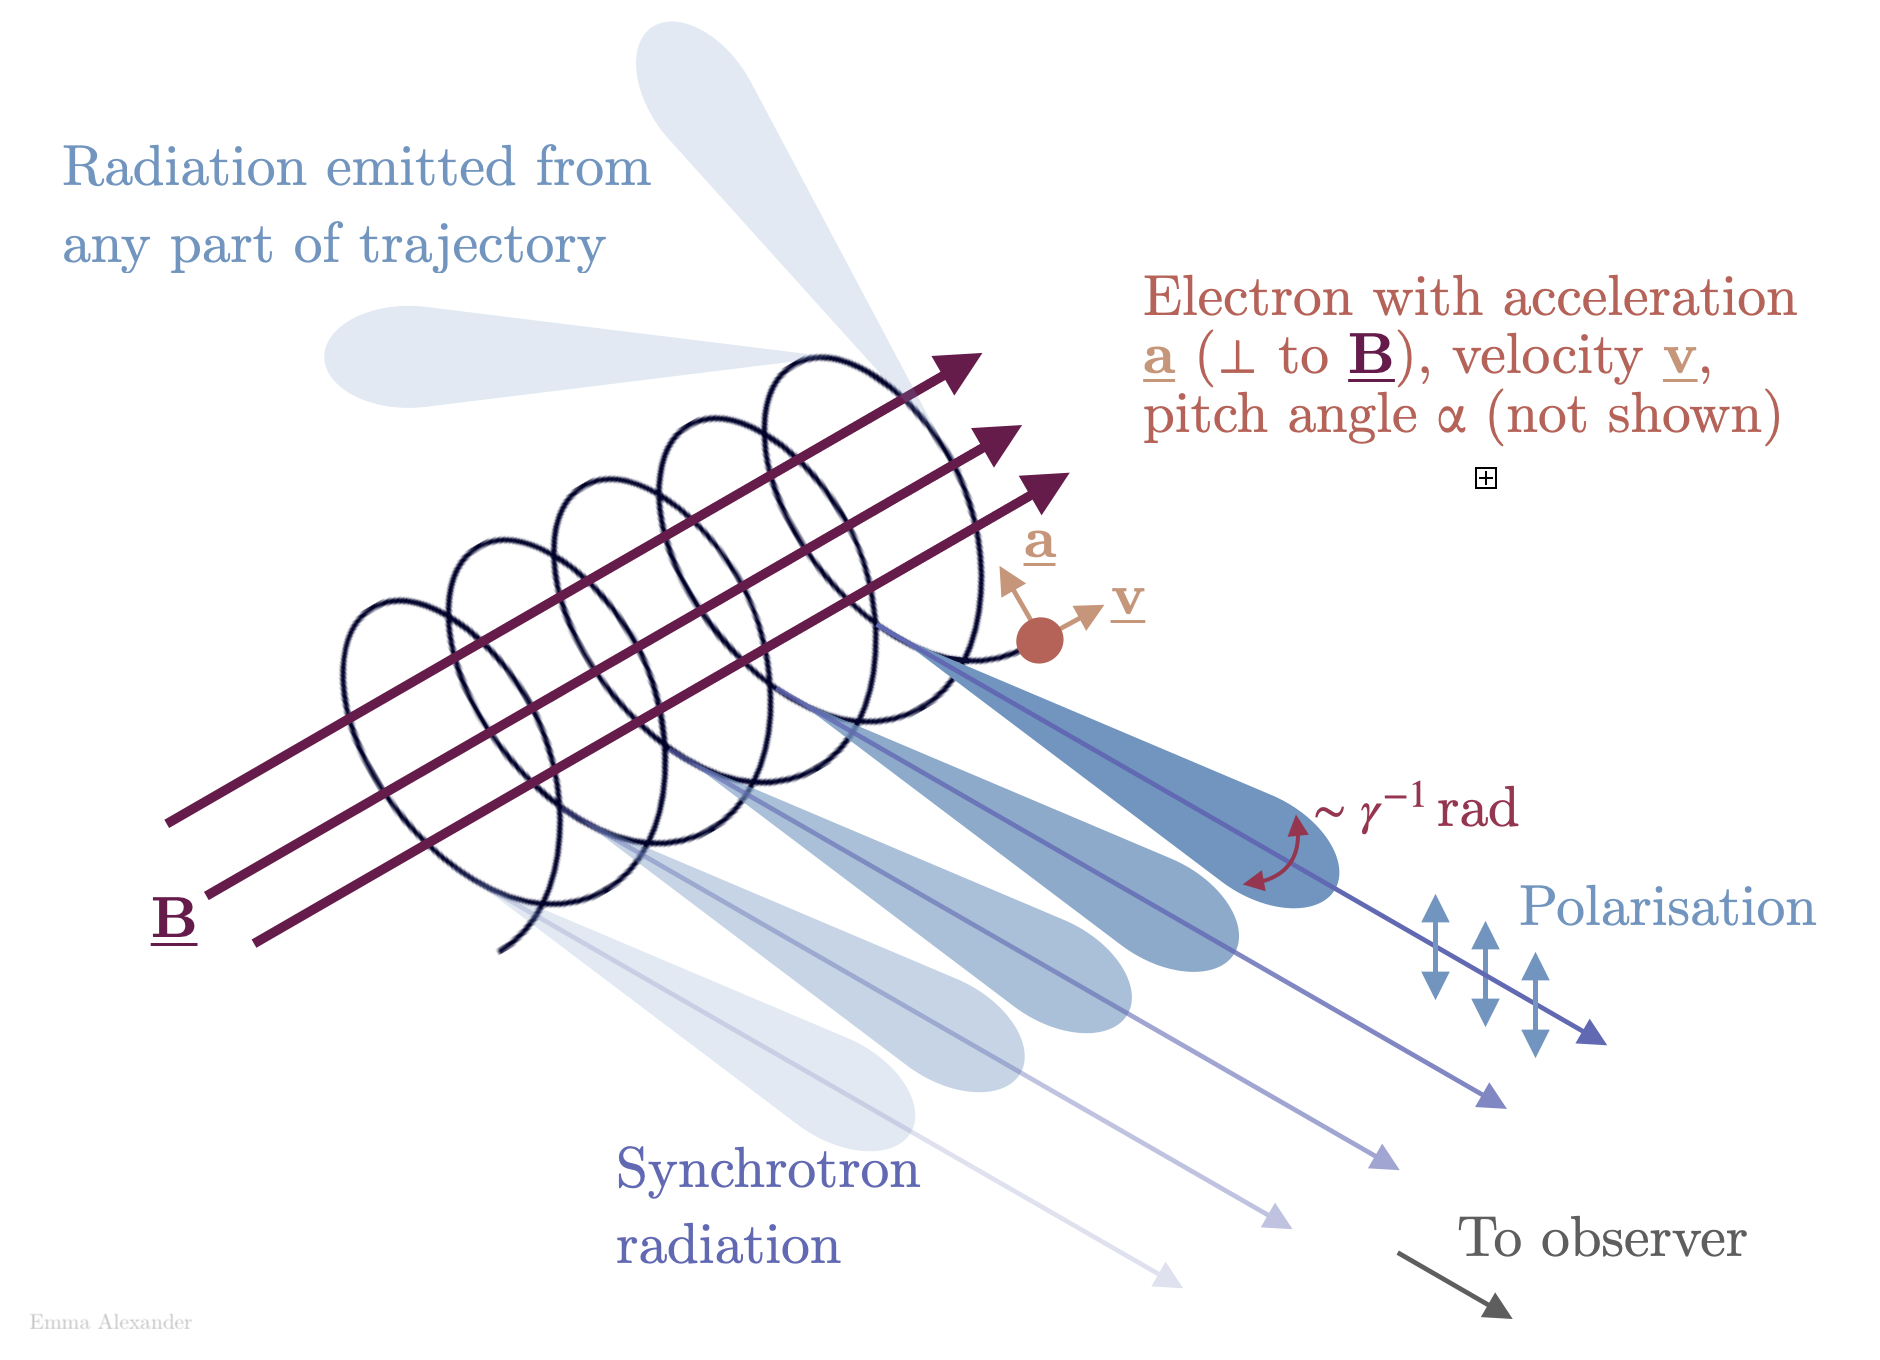
\includegraphics[width=\textwidth, keepaspectratio]{./figures/synchrotron/synchrotron.png}
					\caption{Mecanismo de radiacion sincrotron, Emma Alexander.}
				\end{figure}
			\end{column}
			
			\begin{column}{0.48\textwidth}
				\begin{figure}
					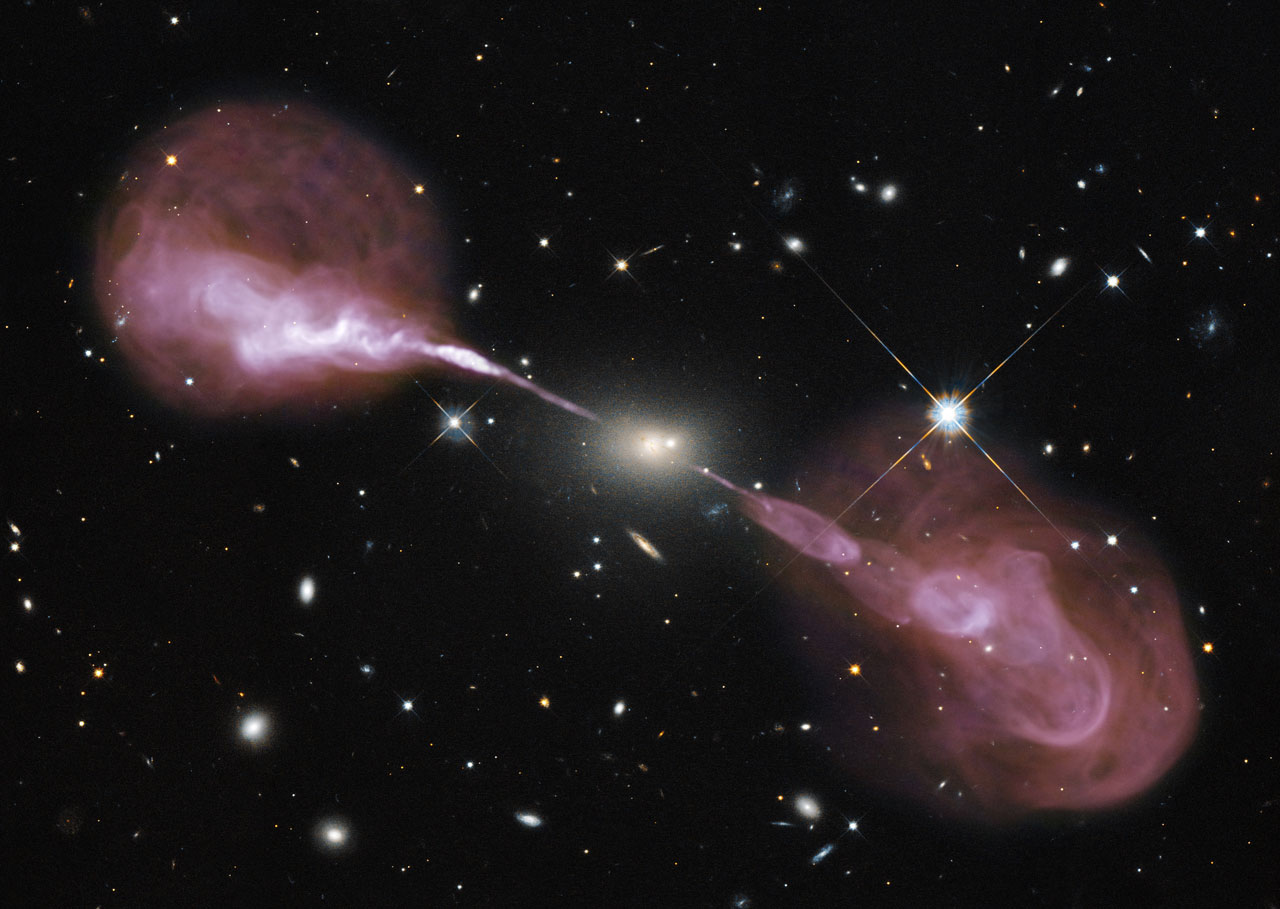
\includegraphics[width=\textwidth, keepaspectratio]{./figures/synchrotron/hercA.jpg}
					\caption{Hercules A, C Band, NASA, ESA, S. Baum and C. O'Dea (RIT), R. Perley and W. Cotton (NRAO/AUI/NSF), and the Hubble Heritage Team (STScI/AURA)}
				\end{figure}
				
				
			\end{column}
		\end{columns}
	\end{frame}

\end{document}
